\documentclass[12pt]{article}


% -------------------- PAQUETES --------------------
\usepackage[utf8]{inputenc}
\usepackage[spanish]{babel}
\usepackage[margin=2.54cm]{geometry}
\usepackage{graphicx}
\usepackage{xcolor}


% -------------------- CARGA DE ARCHIVOS EXTERNOS --------------------
% ----------------- UTILIDADES PARA DAR UN MEJOR FORMATO DE DOCUMENTO -----------------  


\definecolor{azul}{rgb}{0.0039, 0.3098, 0.6196}


% Formato para el indice general ...........
\makeatletter
    \renewcommand{\@dotsep}{1.5}
    \renewcommand{\l@section}{\@dottedtocline{1}{1.5em}{2.3em}}
    \renewcommand{\l@subsection}{\@dottedtocline{2}{3.8em}{3.2em}}
    \renewcommand{\l@subsubsection}{\@dottedtocline{3}{7.0em}{4.1em}}
\makeatother

% --------- COMANDOS PERSONALIZADOS PARA LA PORTADA DE LAS TAREAS, TRABAJOS Y PROYECTOS ---------

\newcommand{\rutaLogo}[1]{\newcommand{\RutaLogo}{#1}}
\newcommand{\tema}[1]{\newcommand{\Tema}{#1}}
\newcommand{\etiquetaAutores}[1]{\newcommand{\EtiquetaAutores}{#1}}
\newcommand{\alumno}[1]{\newcommand{\Alumno}{#1}}
\newcommand{\materia}[1]{\newcommand{\Materia}{#1}}
\newcommand{\docente}[1]{\newcommand{\Docente}{#1}}
\newcommand{\ciclo}[1]{\newcommand{\Ciclo}{#1}}
\newcommand{\fecha}[1]{\newcommand{\Fecha}{#1}}
\newcommand{\periodo}[1]{\newcommand{\Periodo}{#1}}



% -------------------- DEFINICIÓN DE LA PORTADA --------------------
\rutaLogo{../../../../../RecursosGlobales/Img/logo_tec_azuay.png}
\tema{\\ \vspace{1cm} Actividad N°1: Miscelánea de ejercicios de algoritmos secuenciales \\ \vspace{1.7cm}}
\etiquetaAutores{Alumno:}
\alumno{Eduardo Mendieta \vspace{1cm}}
\materia{Introducción a la programación \vspace{1cm}}
\docente{Ing. Verónica Segarra \vspace{1cm}}
\ciclo{Primer Ciclo \vspace{1.1cm}}
\fecha{01 de junio de 2024 \vspace{1cm}}
\periodo{Abril 2024 - Agosto 2024}



% -------------------- INFORME --------------------
\begin{document}

    \begin{titlepage}

    \centering

    \includegraphics[width=0.11\textwidth]{\RutaLogo} 

    \vspace{0.3cm}
    \textcolor{azul}{\Large \textbf{Instituto Superior Universitario Tecnológico del Azuay \\}}
    \vspace{0.3cm}
    \textcolor{azul}{\Large \textbf{Tecnología Superior en Big Data}}
    
    % 1. ---------------- TEMA -------------------------
    
    {\Large\textbf{\Tema}}
    
    % 2. ---------------- AUTOR(ES) -------------------------
    \textcolor{azul}{\large \textbf{\EtiquetaAutores} \\}
    \vspace{0.3cm}
    {\large \Alumno}

    % 3. ---------------- MATERIA -------------------------
    \textcolor{azul}{\large \textbf{Materia:} \\}
    \vspace{0.3cm}
    {\large \Materia}


    % 3. ---------------- DOCENTE -------------------------
    \textcolor{azul}{\large \textbf{Docente:} \\}
    \vspace{0.3cm}
    {\large \Docente}


    % 3. ---------------- Ciclo -------------------------
    \textcolor{azul}{\large \textbf{Ciclo:} \\}
    \vspace{0.3cm}
    {\large \Ciclo}


    % 3. ---------------- FECHA -------------------------
    \textcolor{azul}{\large \textbf{Fecha:} \\}
    \vspace{0.3cm}
    {\large \Fecha}

    % 3. ---------------- PERIODO -------------------------
    \textcolor{azul}{\large \textbf{Periodo Académico:} \\}
    \vspace{0.3cm}
    {\large \Periodo}
 
\end{titlepage}

  
    \section*{\centering Actividad N°1}

        \textbf{Para los siguientes ejercicios, desarrollar: Diagrama de flujo, pruebas de escritorio y algoritmo en PseInt.}

        \begin{enumerate}
            % Ejercicio 1: -----------------------------------------------
            \item  Pidiendo el ingreso del numerador y denominador de 2 fracciones mostrar la suma.
            
                \begin{figure}[!h]
                    \centering
                    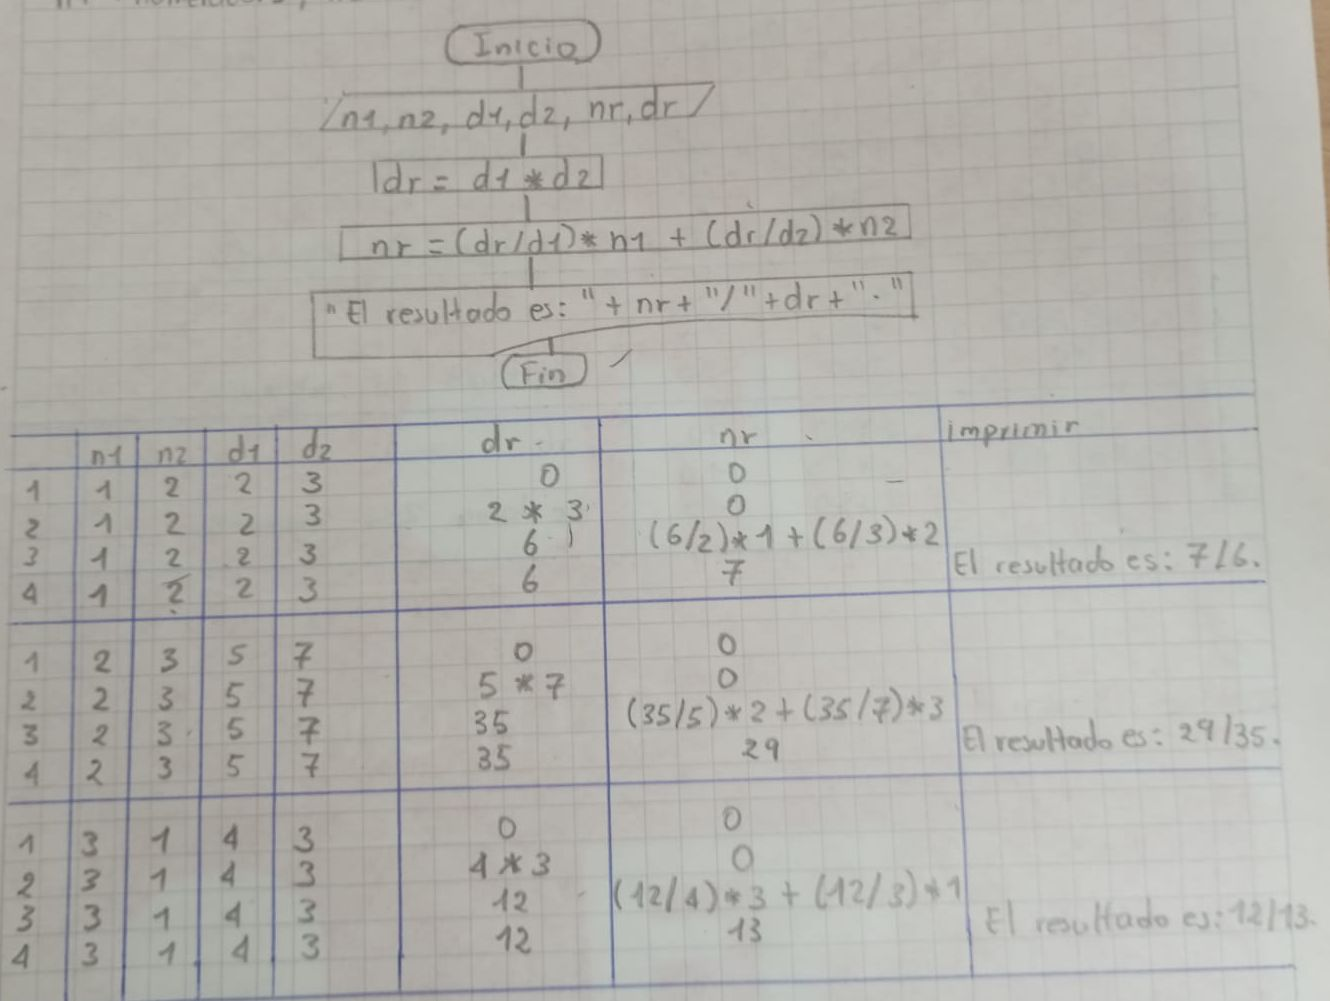
\includegraphics[width=0.9\textwidth]{Img/DF_ej1.jpeg}
                \end{figure}

                \begin{figure}[!h]
                    \centering
                    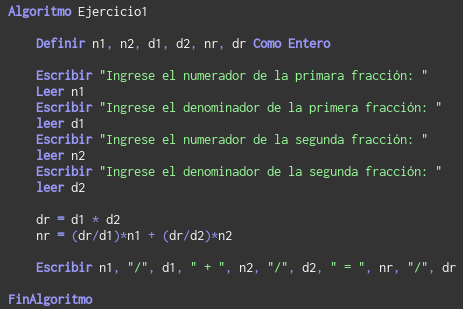
\includegraphics[width=0.6\textwidth]{Img/Cod_ej1.png}
                \end{figure}

                \begin{figure}[!h]
                    \centering
                    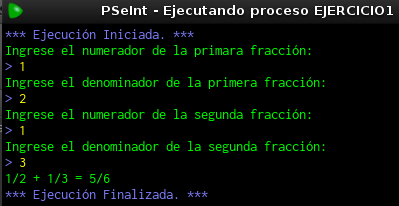
\includegraphics[width=0.5\textwidth]{Img/Ejec_ej1.png}
                \end{figure}

            % Ejercicio 2: -----------------------------------------------
            \item Se requiere determinar el tiempo que tarda una persona en llegar de una ciudad a otra en bicicleta, considerando que lleva una velocidad constante. Realice un diagrama de flujo y pseudocódigo que representen el algoritmo para tal fin.
            
                \begin{figure}[!h]
                    \centering
                    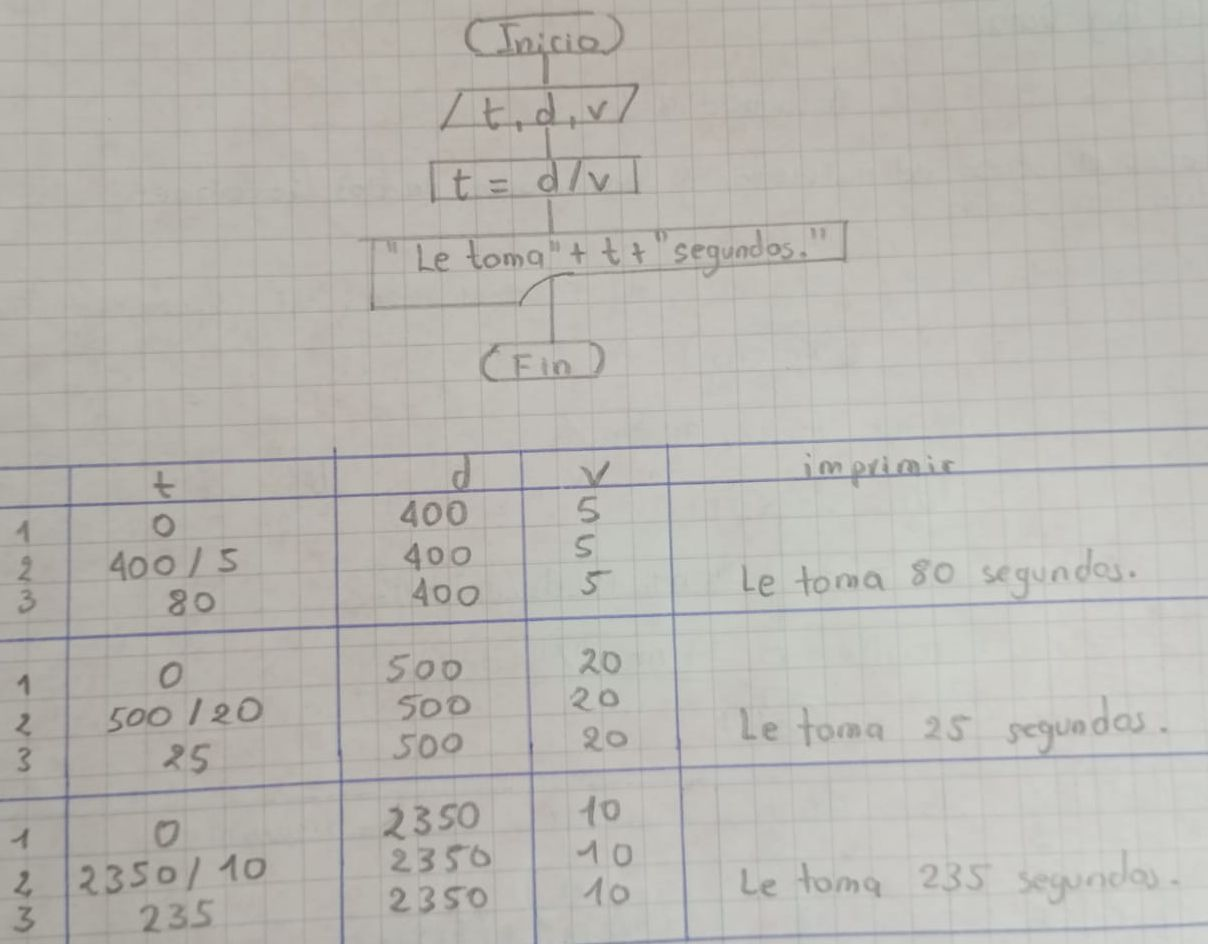
\includegraphics[width=0.9\textwidth]{Img/DF_ej2.jpeg}
                \end{figure}

                \newpage
                \begin{figure}[!h]
                    \centering
                    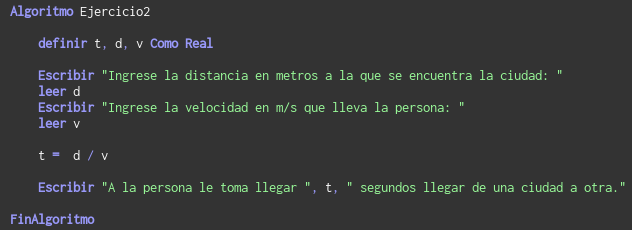
\includegraphics[width=0.9\textwidth]{Img/Cod_ej2.png}
                \end{figure}

                \begin{figure}[!h]
                    \centering
                    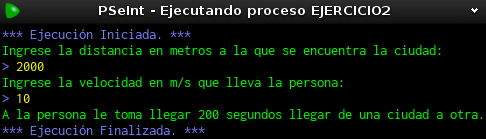
\includegraphics[width=0.6\textwidth]{Img/Ejec_ej2.png}
                \end{figure}

            % Ejercicio 3: -----------------------------------------------
            \item Realizar un algoritmo que calcule la potencia de un número real elevado a un número natural.
            
                \begin{figure}[!h]
                    \centering
                    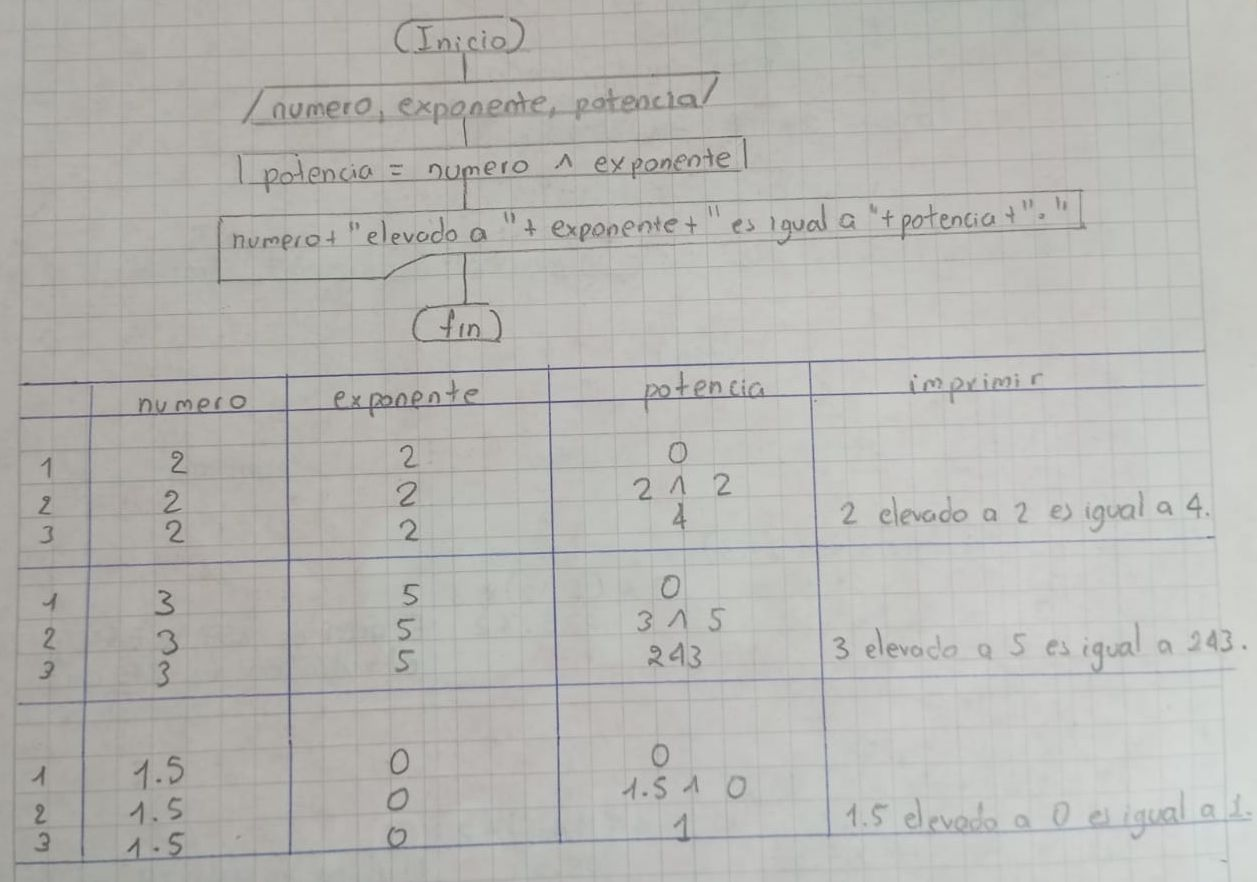
\includegraphics[width=0.9\textwidth]{Img/DF_ej3.jpeg}
                \end{figure}

                \newpage
                \begin{figure}[!h]
                    \centering
                    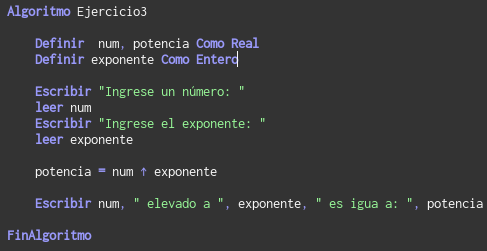
\includegraphics[width=0.7\textwidth]{Img/Cod_ej3.png}
                \end{figure}

                \begin{figure}[!h]
                    \centering
                    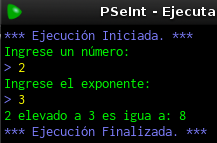
\includegraphics[width=0.35\textwidth]{Img/Ejec_ej3.png}
                \end{figure}
            
            % Ejercicio 4: -----------------------------------------------
            \newpage
            \item Diseñar un algoritmo que determine el área y el volumen de un cilindro.
            
                \begin{figure}[!h]
                    \centering
                    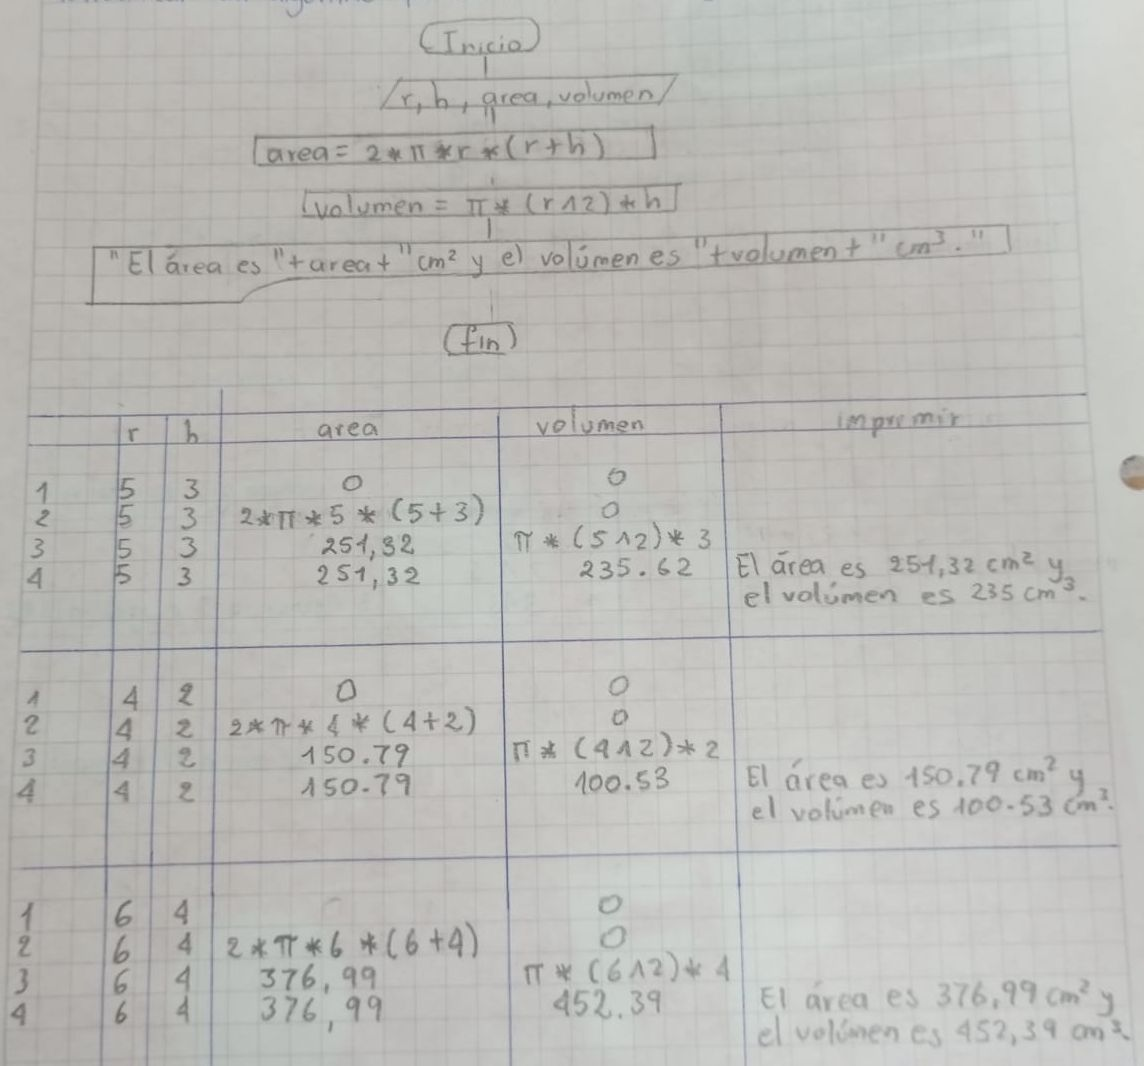
\includegraphics[width=0.9\textwidth]{Img/DF_ej4.jpeg}
                \end{figure}

                \begin{figure}[!h]
                    \centering
                    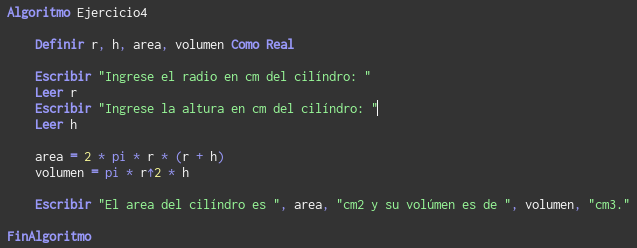
\includegraphics[width=0.8\textwidth]{Img/Cod_ej4.png}
                \end{figure}

                \newpage
                \begin{figure}[!h]
                    \centering
                    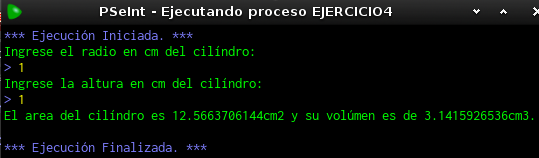
\includegraphics[width=0.7\textwidth]{Img/Ejec_ej4.png}
                \end{figure}
                
            % Ejercicio 5: -----------------------------------------------
            \newpage
            \item Una empresa desea determinar el monto de un cheque que debe  proporcionar a uno de sus empleados que tendrá que ir por equis número de días a la ciudad de Quito; los gastos que cubre la empresa son: hotel, comida y \$100.00 dólares diarios para otros gastos. El monto debe estar desglosado para cada concepto. Realice un diagrama de flujo que representen el algoritmo que determine el monto del cheque.
            
                \begin{figure}[!h]
                    \centering
                    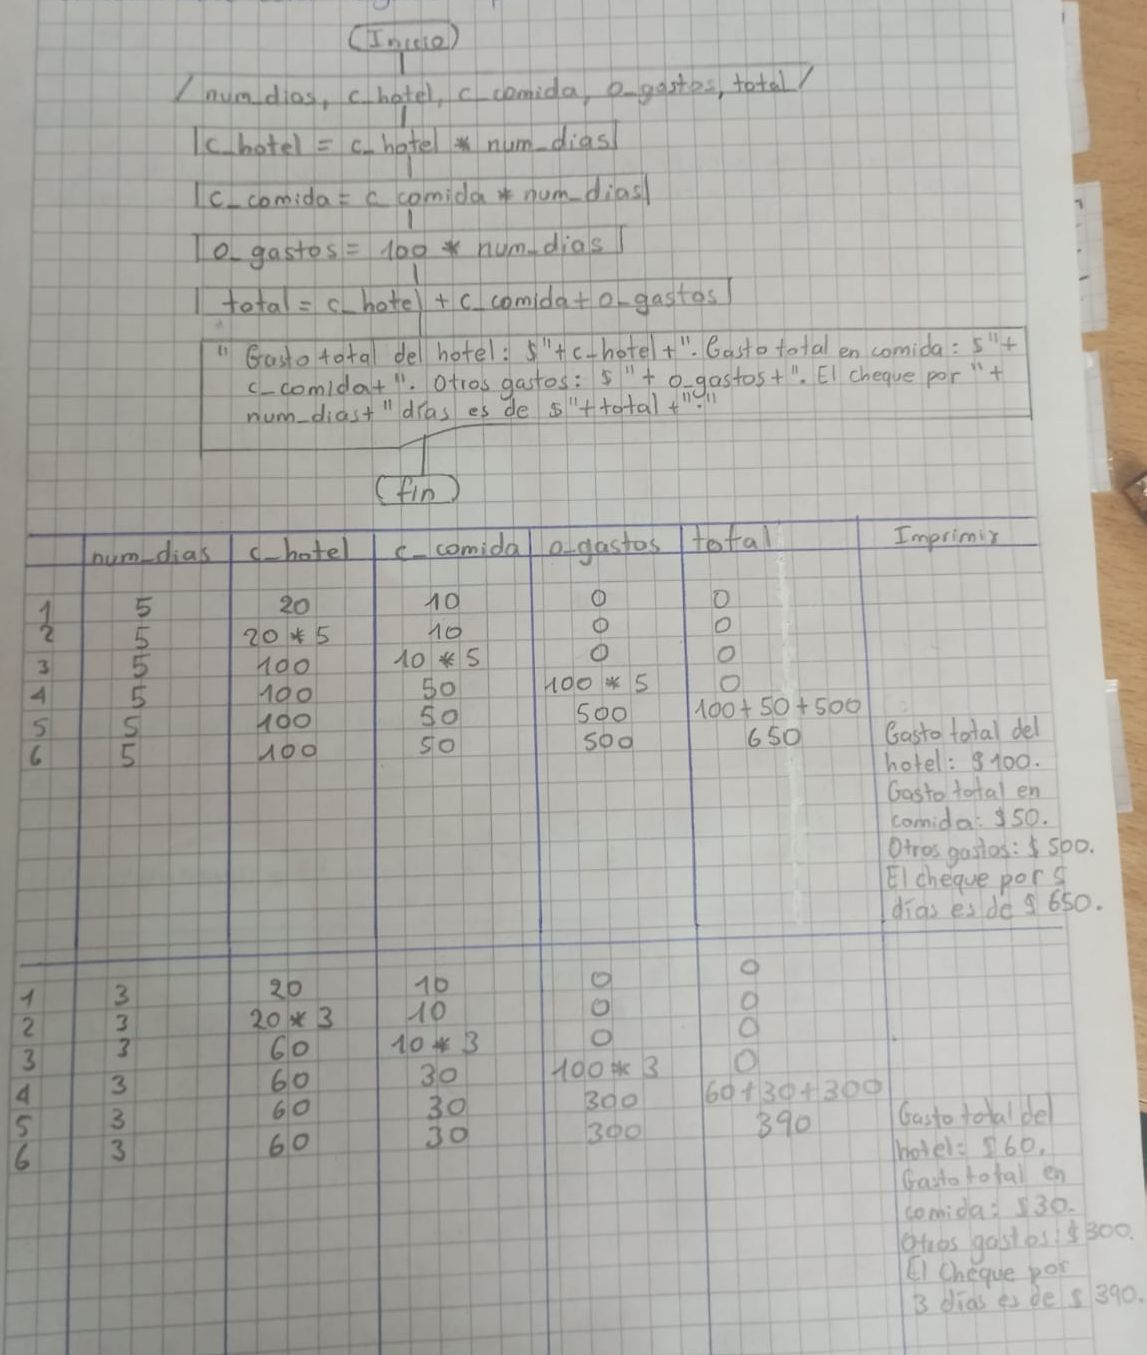
\includegraphics[width=0.9\textwidth]{Img/DF_ej5.jpeg}
                \end{figure}

                \newpage
                \begin{figure}[!h]
                    \centering
                    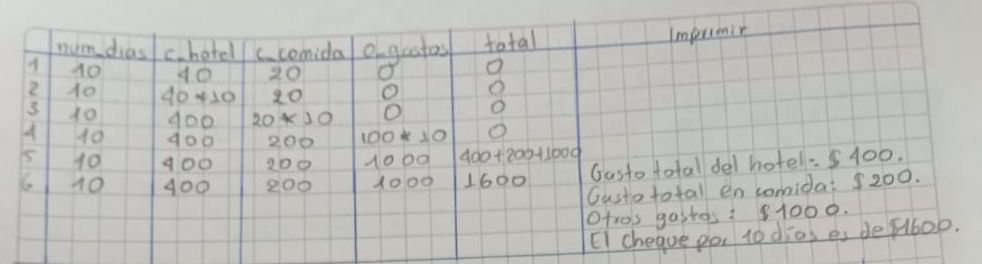
\includegraphics[width=0.9\textwidth]{Img/DF_ej5_2.jpeg}
                \end{figure}

                \begin{figure}[!h]
                    \centering
                    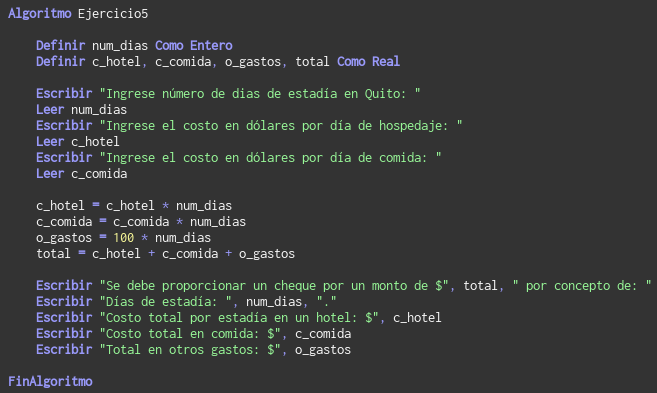
\includegraphics[width=0.8\textwidth]{Img/Cod_ej5.png}
                \end{figure}

                \begin{figure}[!h]
                    \centering
                    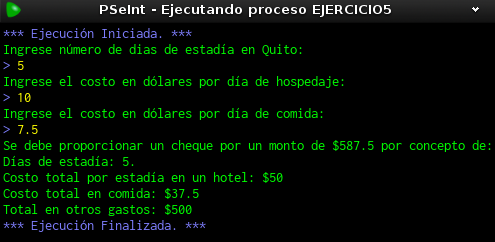
\includegraphics[width=0.6\textwidth]{Img/Ejec_ej5.png}
                \end{figure}
            
            % Ejercicio 6: -----------------------------------------------
            \newpage
            \item Una empresa que contrata personal requiere determinar la edad de las   personas que solicitan trabajo, pero cuando se les realiza la entrevista sólo  se les pregunta el año en que nacieron. Realice el diagrama de flujo y  pseudocódigo que representen el algoritmo para solucionar este problema.
            
                \begin{figure}[!h]
                    \centering
                    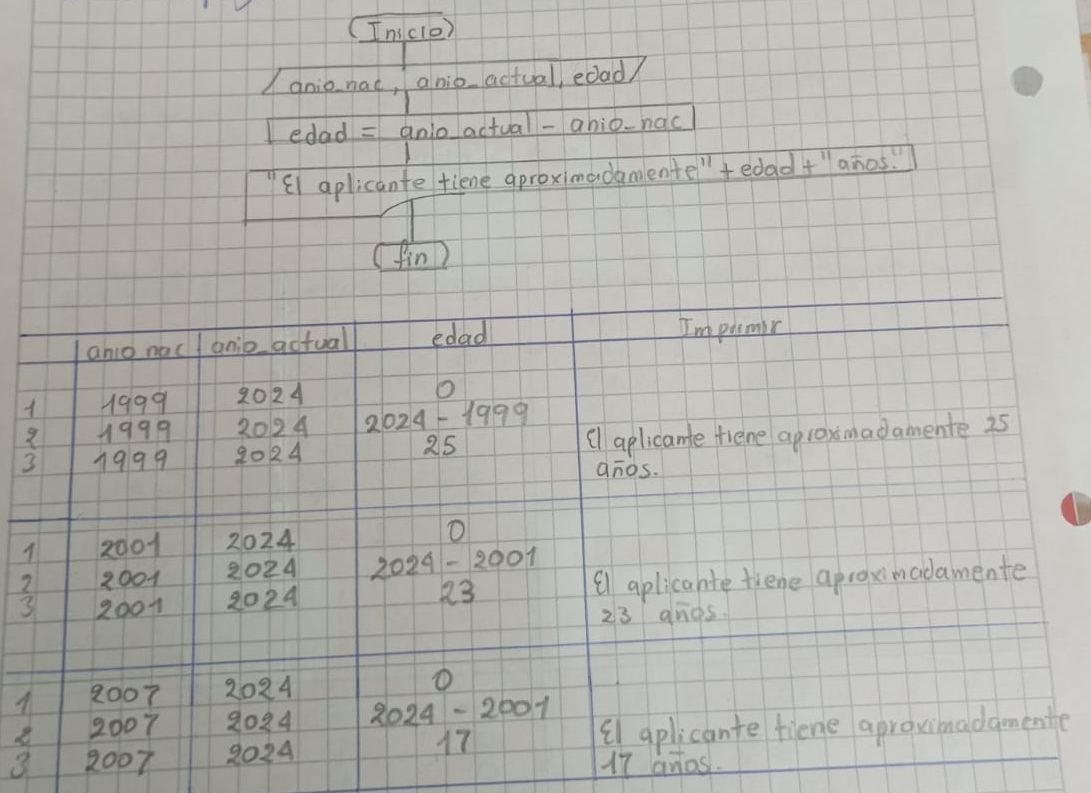
\includegraphics[width=0.9\textwidth]{Img/DF_ej6.jpeg}
                \end{figure}

                \begin{figure}[!h]
                    \centering
                    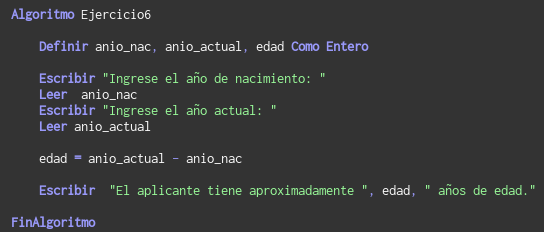
\includegraphics[width=0.7\textwidth]{Img/Cod_ej6.png}
                \end{figure}

                \begin{figure}[!h]
                    \centering
                    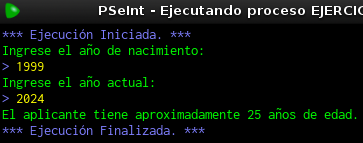
\includegraphics[width=0.5\textwidth]{Img/Ejec_ej6.png}
                \end{figure}
            
            % Ejercicio 7: -----------------------------------------------
            \newpage
            \item Se requiere determinar la hipotenusa de un triángulo rectángulo. ¿Cómo   sería el diagrama de flujo y el pseudocódigo que representen el algoritmo    para obtenerla? Recuerde que por Pitágoras se tiene que: C2 = A2 + B2.
           
                \begin{figure}[!h]
                    \centering
                    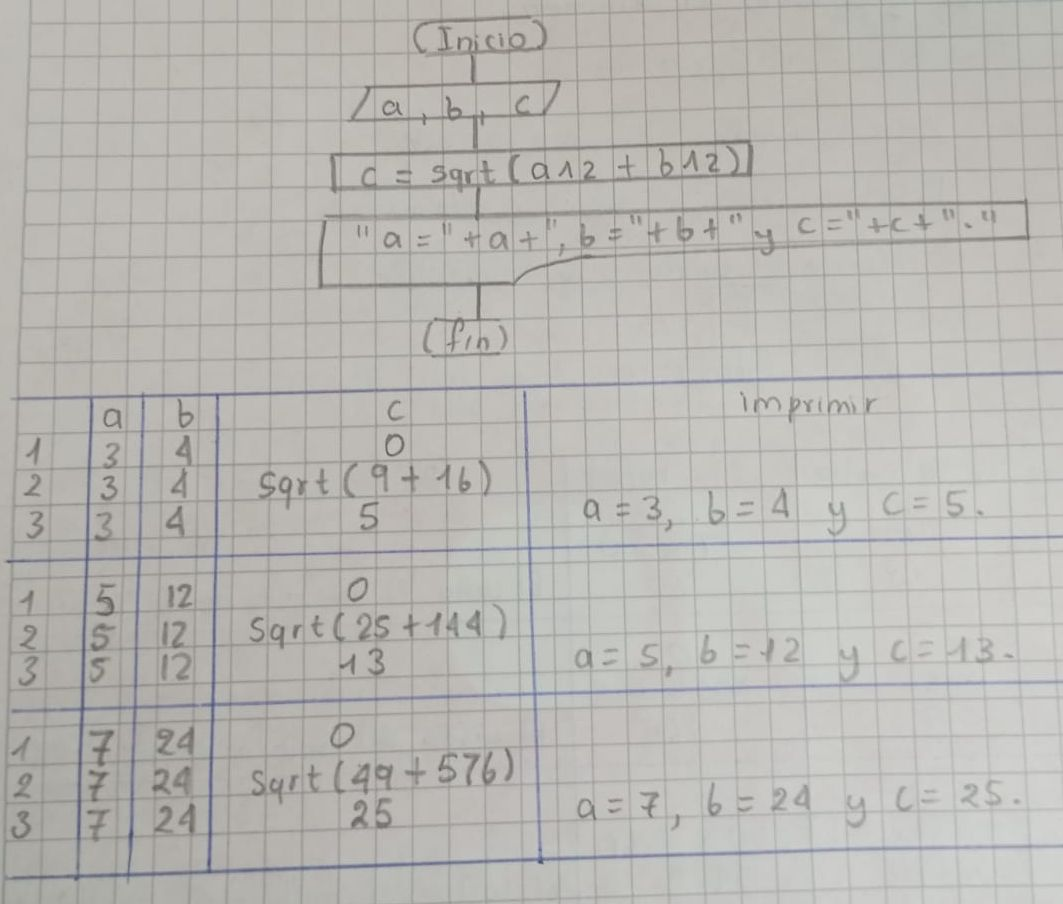
\includegraphics[width=0.9\textwidth]{Img/DF_ej7.jpeg}
                \end{figure}

                \begin{figure}[!h]
                    \centering
                    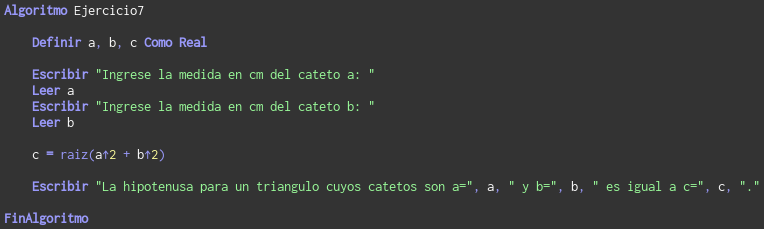
\includegraphics[width=0.8\textwidth]{Img/Cod_ej7.png}
                \end{figure}

                \begin{figure}[!h]
                    \centering
                    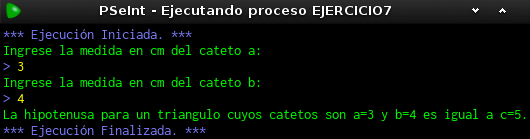
\includegraphics[width=0.6\textwidth]{Img/Ejec_ej7.png}
                \end{figure}
            
            % Ejercicio 8: -----------------------------------------------
            \newpage
            \item La compañía de autobuses “La curva loca” requiere determinar el costo que  tendrá el boleto de un viaje sencillo, esto basado en los kilómetros por  recorrer y en el costo por kilómetro. Realice un diagrama de flujo y pseudocódigo que representen el algoritmo para tal fin.
           
                \begin{figure}[!h]
                    \centering
                    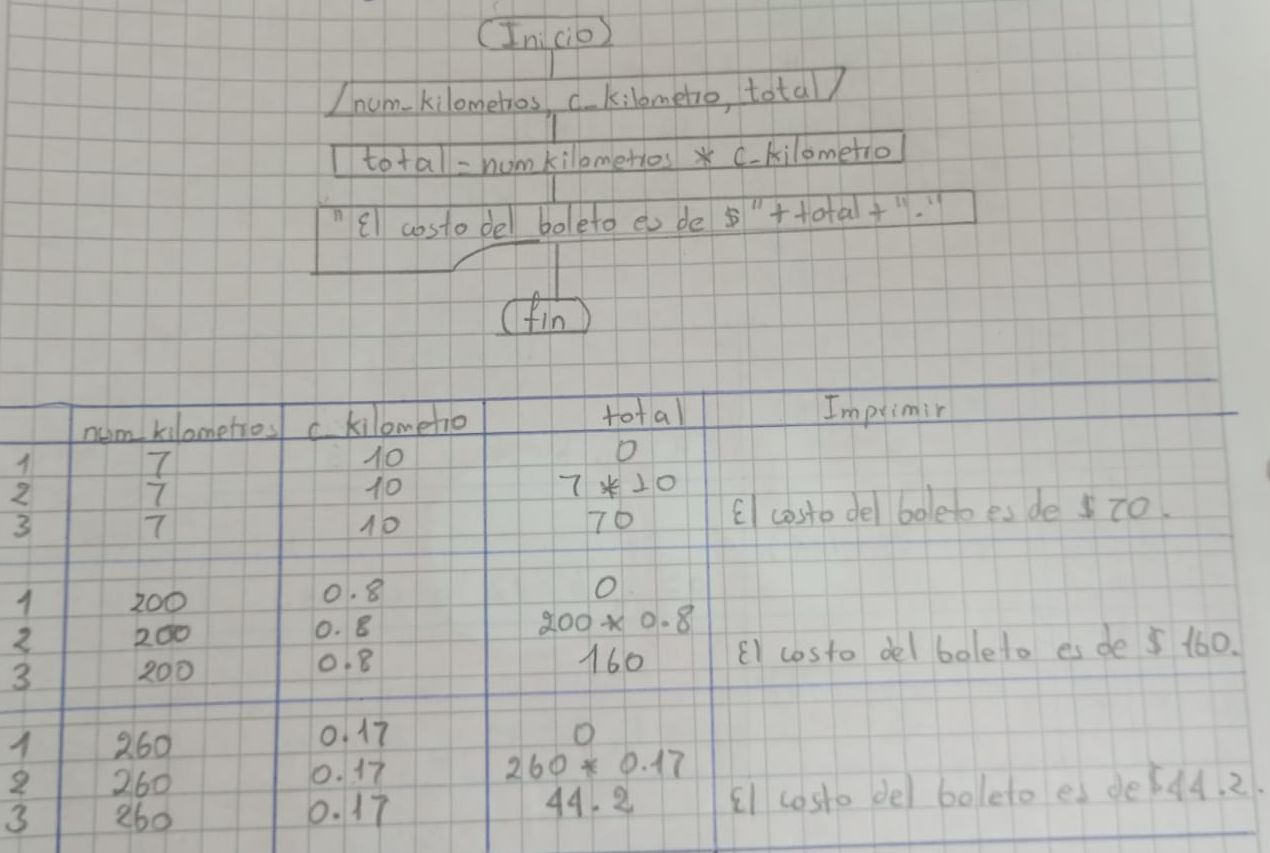
\includegraphics[width=0.9\textwidth]{Img/DF_ej8.jpeg}
                \end{figure}

                \newpage
                \begin{figure}[!h]
                    \centering
                    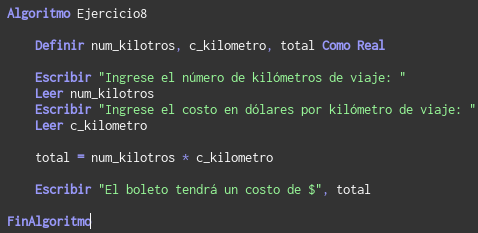
\includegraphics[width=0.8\textwidth]{Img/Cod_ej8.png}
                \end{figure}

                \begin{figure}[!h]
                    \centering
                    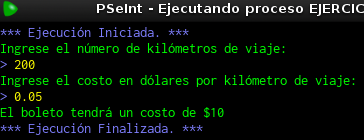
\includegraphics[width=0.6\textwidth]{Img/Ejec_ej8.png}
                \end{figure}
           
            % Ejercicio 9: -----------------------------------------------
            \newpage
            \item Realice un diagrama de flujo que representen el algoritmo para determinar cuánto pagará finalmente una persona por un artículo equis, considerando  que tiene un descuento de 20\%, y debe pagar 12\% de IVA (debe mostrar el  precio con descuento y el precio final).
            
                \begin{figure}[!h]
                    \centering
                    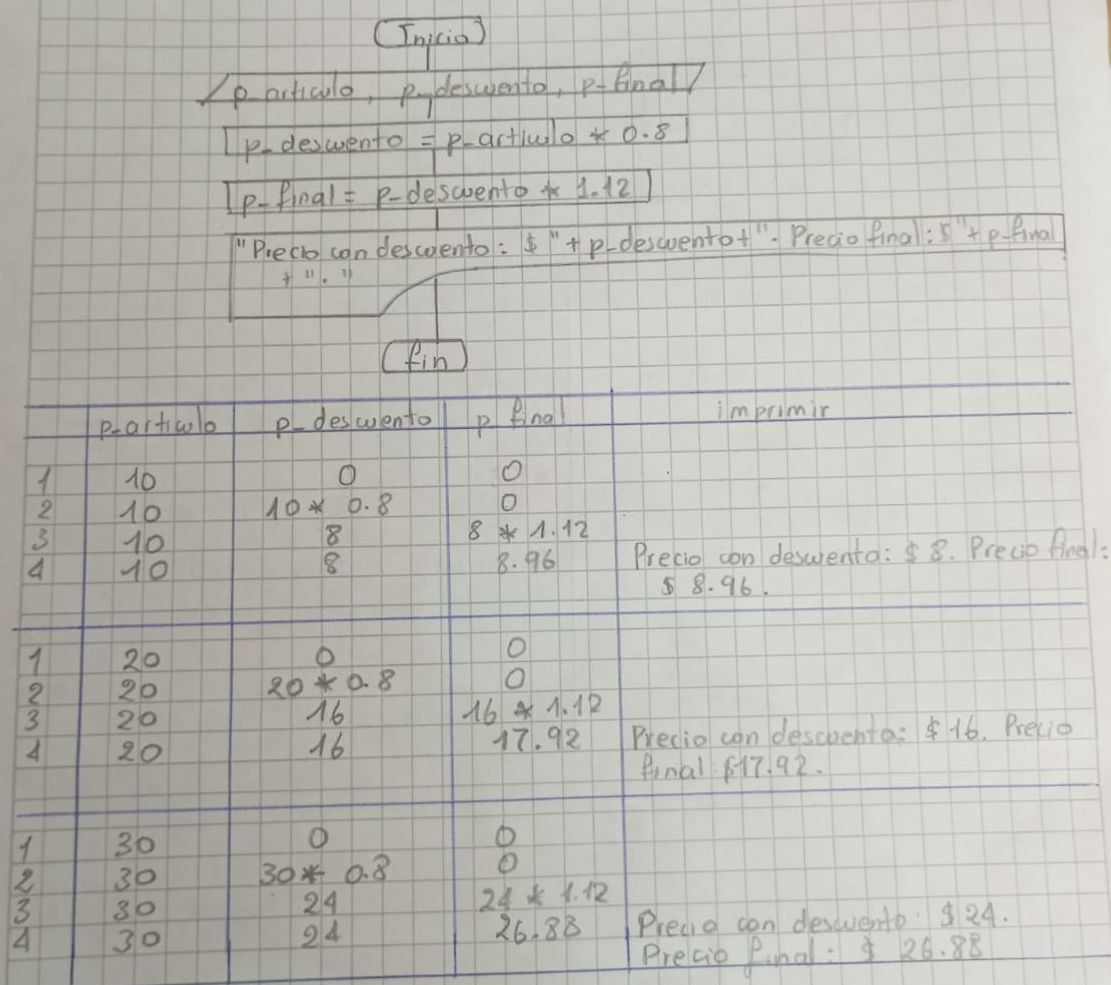
\includegraphics[width=0.9\textwidth]{Img/DF_ej9.jpeg}
                \end{figure}

                \begin{figure}[!h]
                    \centering
                    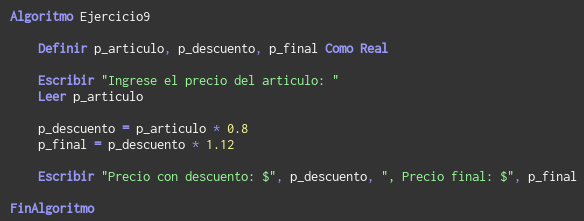
\includegraphics[width=0.8\textwidth]{Img/Cod_ej9.png}
                \end{figure}

                \newpage
                \begin{figure}[!h]
                    \centering
                    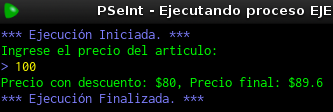
\includegraphics[width=0.6\textwidth]{Img/Ejec_ej9.png}
                \end{figure}
            
            % Ejercicio 10: -----------------------------------------------
            \item Realice un diagrama de flujo que representen el algoritmo para determinar cuánto dinero ahorra una persona en un año si considera que cada semana ahorra 15\% de su sueldo (considere cuatro semanas por mes y que no cambia el sueldo).
        
                \begin{figure}[!h]
                    \centering
                    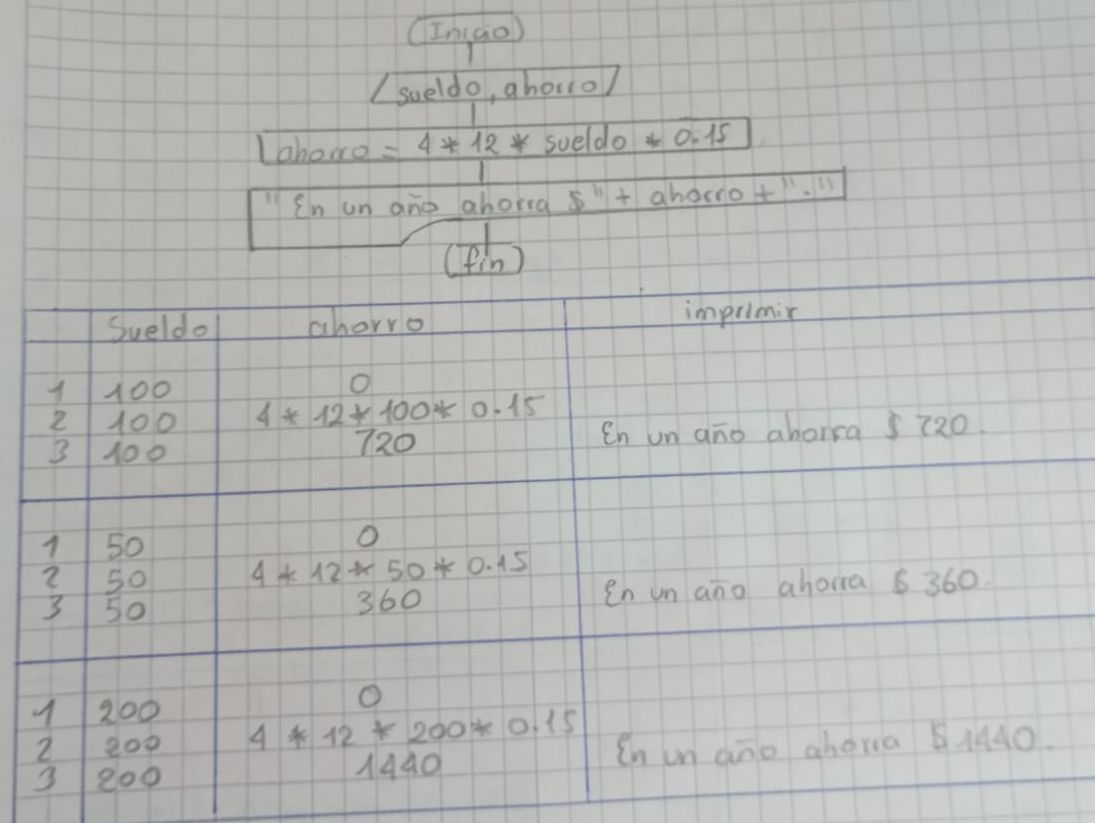
\includegraphics[width=0.9\textwidth]{Img/DF_ej10.jpeg}
                \end{figure}

                \newpage
                \begin{figure}[!h]
                    \centering
                    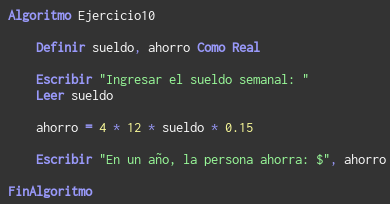
\includegraphics[width=0.6\textwidth]{Img/Cod_ej10.png}
                \end{figure}

                \begin{figure}[!h]
                    \centering
                    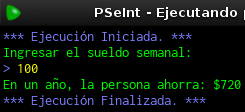
\includegraphics[width=0.4\textwidth]{Img/Ejec_ej10.png}
                \end{figure}
        
        \end{enumerate}

\end{document}